\subsection{Algoritmos implementados}
\fontsize{8pt}{0}\selectfont
 \begin{frame}\frametitle{MWMOTE}
  \vspace{2em}
  \begin{algorithmic}[1]
    \REQUIRE $\spos = \{x_1, \ldots x_m\}$, clase minoritaria
    \REQUIRE $\sneg = \{y_1, \ldots y_m\}$, clase mayoritaria
    \REQUIRE $T$, número de instancias sintéticas deseado
    \REQUIRE $k_{1}, k_{2}, k_{3}$, parámetros de KNN para filtrar ruido de $\spos$ y calcular fronteras.
    \REQUIRE $\alpha$, umbral de tolerancia en la cercanía a la frontera
    \REQUIRE $C$, ponderación cercanía a la frontera, $C_{clust}$, para determinar número de clústers
    \STATE{Hacer $\spos_f = \spos - \{x\in \spos : NN^{k_1}(x) \cap \spos = \emptyset\}$}
    \STATE{Calcular fronteras negativa $U = \underset{x\in \spos_f}{\bigcup} NN_{-}^{k_2}(x)$ y 
    positiva $V = \underset{x\in U}{\bigcup} NN_{+}^{k_3}(x)$}
    \STATE{Para cada $x\in V$, calcular $P(x) = \sum_{y\in U} I_{\alpha,C}(x,y)$}
    \STATE{Normalizar para cada $x\in V$, $P(x) = \frac{P(x)}{\sum_{z\in V} P(z)}$}
    \STATE{Calcular $T_{clust} = C_{clust} \cdot \frac{1}{|\spos_f|} \sum_{x\in \spos_f} \min_{y\in \spos_f, y\neq x} d(x,y)$}
    \STATE{Calcular $L_1, \ldots L_M\subseteq \spos$ clústers para $\spos$, con umbral $T_{clust}$}
    \FOR{$t=1, \ldots, T$}
      \STATE{Escoger $x\in V$ de acuerdo a la probabilidad $P(x)$}
      \STATE{Seleccionar $y\in L_k$ uniformemente donde $L_k \ni x$ ($L_k$ es el clúster de $x$)}
      \STATE{Seleccionar $r$ en $[0,1]$ de manera uniforme}
      \STATE{$S' = S'\cup \{x + r(y-x)\}$}
    \ENDFOR
    \RETURN{$S'$, ejemplos positivos sintéticos}
  \end{algorithmic}
 \end{frame}

 \begin{frame}\frametitle{SMOTE vs MWMOTE}
 \begin{center}
   \begin{overprint}
   \onslide<1> \vspace{2cm} \centering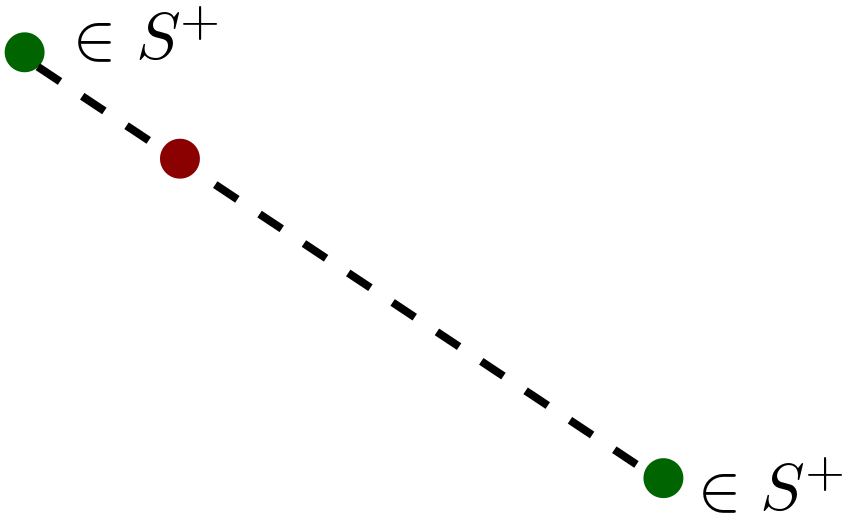
\includegraphics[scale=0.25]{imgs/smote.png}
   \onslide<2> \vspace{1.12cm} \hspace{-0.65cm}\centering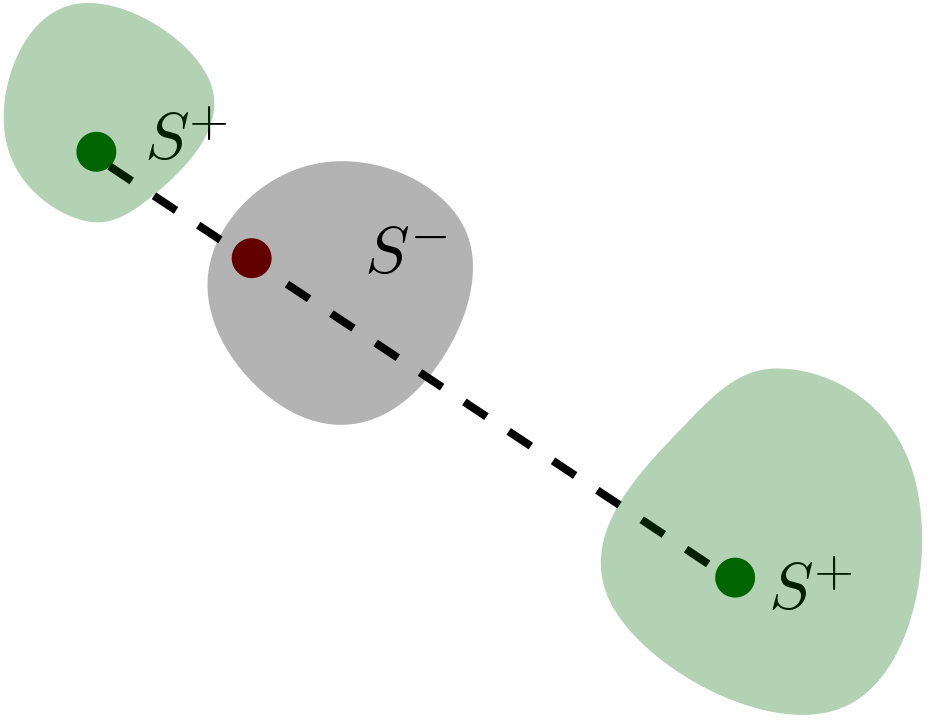
\includegraphics[scale=0.25]{imgs/smote-flaws.png}
   \onslide<3> \vspace{1.12cm} \hspace{-0.65cm}\centering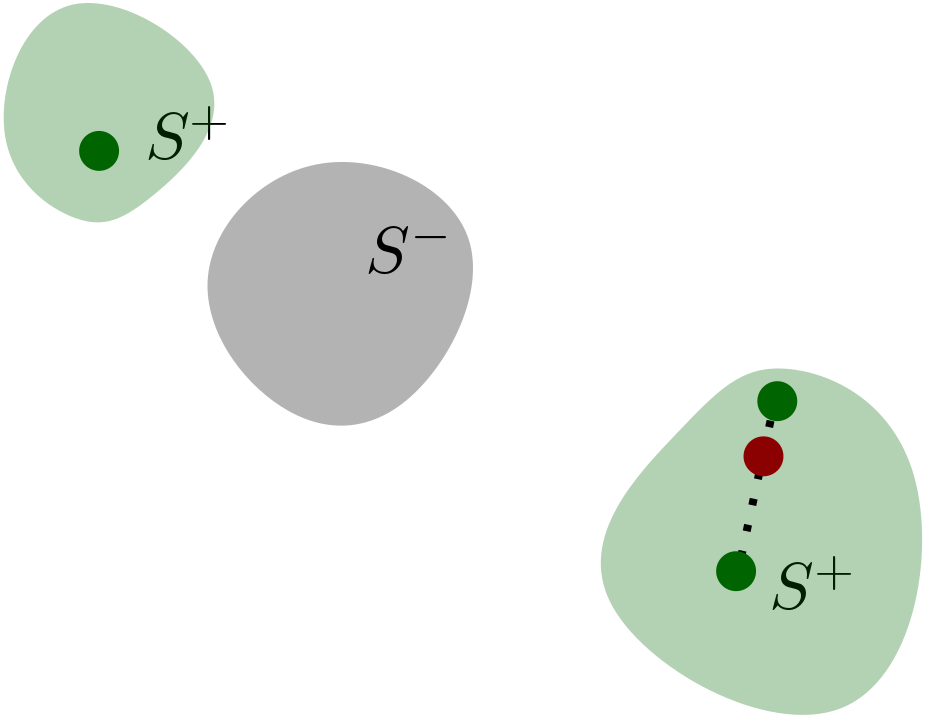
\includegraphics[scale=0.25]{imgs/mwmote-clusters.png}
  \end{overprint}
 \end{center}
 \end{frame}
 
 \begin{frame}\frametitle{RACOG y wRACOG}
 \vspace{2em}
 \begin{columns}
  \begin{column}{0.45\textwidth}
   \begin{algorithmic}[1]
     \REQUIRE $S = \{x_1, \ldots x_m\}$, ejemplos positivos
     \REQUIRE $\beta$, burnin
     \REQUIRE $\alpha$, lag
     \REQUIRE $T$, número de instancias sintéticas a generar
     \STATE{$P = \textrm{AproximarDistribución}(S)$}
     \STATE{$S'= \emptyset$}
     \STATE{$M = \left\lceil\frac{T}{m}\right\rceil \cdot \alpha + \beta$}
     \FOR{$t=1,\ldots, M$}
       \STATE{$S = \textrm{GibbsSampler}(S, P)$}
       \IF{$t > \beta$ \AND $t\mod(\alpha) = 0$}
         \STATE{$S' = S' \cup S$}
       \ENDIF
     \ENDFOR
     \STATE{$S' =$ Escoger $T$ instancias desde $S'$}
     \RETURN{$S'$, ejemplos positivos sintéticos}    
   \end{algorithmic}
  \end{column}
  
  \begin{column}{0.6\textwidth}
   \begin{algorithmic}[1]
    \REQUIRE $S_{train} = \{z_i=(x_i, y_i)\}_{i=1}^m$
    \REQUIRE $S_{val}$, conjunto de validación
    \REQUIRE $wrapper$, clasificador
    \REQUIRE $T$, número de iteraciones a considerar
    \REQUIRE $\alpha$, parámetro de tolerancia
    \STATE{$S = \spos_{train}$}
    \STATE{$P = \textrm{AproximarDistribución}(S)$}
    \STATE{Obtener $modelo$ con $wrapper$ y $S_{train}$}
    \STATE{Inicializar nuevas muestras $S'= \emptyset$}
    \STATE{Inicializar $\tau = (\underset{1)}{+\infty}, \ldots, \underset{T)}{+\infty})$}
    \WHILE{Desviación estándar de $\tau \ge \alpha$}
      \STATE{$S = \textrm{GibbsSampler}(S, P)$}
      \STATE{$S_{misc} =$ instancias mal clasificadas de $S$ por $modelo$}
      \STATE{Actualizar nuevas instancias, $S' = S' \cup S_{misc}$}
      \STATE{Actualizar \textit{train}, $S_{train} = S_{train} \cup S_{misc}$}
      \STATE{Obtener $modelo$ con $wrapper$ y $S_{train}$}
      \STATE{Hacer $s = $ sensibilidad de la predicción de $modelo$ sobre $S_{val}$}
      \STATE{Hacer $\tau = (\tau_2, \ldots, \tau_T, s)$}
    \ENDWHILE
    \RETURN{$S'$, ejemplos positivos sintéticos}    
   \end{algorithmic}
  \end{column}
 \end{columns}
 \end{frame}

 \begin{frame}\frametitle{RACOG y wRACOG}
  \vspace{2em}
  \textbf{\large{Idea}}: Aproximar $P(W_1, \ldots, W_d)$ como producto de distribuciones marginales, es decir:
  \[P(W_1, \ldots, W_d) \approx \prod_{i=1}^d P(W_i \mid W_{n(i)})\]
  donde cada $n(i) \in \{1, \ldots, d\}$.
  \begin{columns}
   \begin{column}{0.6\textwidth}
    \img{imgs/chow-liu.png}{1}
   \end{column}

   \begin{column}{0.4\textwidth}
    \img{../memoria/imgs/monte-carlo.png}{1}
   \end{column}
  \end{columns}
 \end{frame}
 
 
 \begin{frame}\frametitle{RWO}
  \vspace{2em}
  \begin{algorithmic}[1]
   \REQUIRE $S = \{x_i=(w_1^{(i)}, \ldots w_d^{(i)})\}_{i=1}^m$, ejemplos positivos
   \REQUIRE $T$, número de instancias sintéticas deseado
   \FOR{Cada atributo $j=1, \ldots, d$}
     \IF{El atributo $j-$ésimo es numérico}
       \STATE{Calcular $\sigma_j'^2 = 1/m \sum_{i=1}^m \left(w_j^{(i)} - 1/m \sum_{i=1}^m w_j^{(i)} \right)^2$}
     \ENDIF
   \ENDFOR
   \STATE{Hacer $M = \left\lceil T/m \right\rceil$}
   \FOR{$t=1, \ldots, M$}
     \FOR{$i=1,\ldots, m$}
       \FOR{$j=1, \ldots, d$}
          \IF{El atributo $j-$ésimo es numérico}
            \STATE{Escoger $r \sim N(0,1)$ y $w_j = w_j^{(i)} - \frac{\sigma_j'}{\sqrt{m}} \cdot r$}
          \ELSE
            \STATE{Escoger $w_j$ de manera uniforme sobre $\{w_j^{(1)}, \ldots w_j^{(m)}\}$}
          \ENDIF
       \ENDFOR
       \STATE{$S' = S' \cup \{(w_1, \ldots w_d)\}$}
     \ENDFOR
   \ENDFOR
   \STATE{$S'=$ Escoger $T$ instancias aleatorias de entre $S'$}
   \RETURN{$S'$, ejemplos positivos sintéticos}
  \end{algorithmic}
 \end{frame}
 
 \begin{frame}\frametitle{PDFOS}
  \begin{columns}
   \begin{column}{0.55\textwidth}
    \imgcaption{../memoria/imgs/kernel-estimation.png}{Estimación de densidades, ejemplo extraído de Wikimedia Commons}{1}
   \end{column}
   
   \begin{column}{0.6\textwidth}
    \begin{algorithmic}[1]
     \REQUIRE $S = \{x_i=(w_1^{(i)}, \ldots w_d^{(i)})\}_{i=1}^m$, ejemplos positivos
     \REQUIRE $T$, número de instancias sintéticas
     \STATE{Inicializamos $S'= \emptyset$}
     \STATE{Búsqueda de $h =$ que minimice $M(h)$}
     \STATE{Calcular $U$ la matriz de covarianza insesgada de $S$}
     \STATE{Calcular descomposición de Choleski de $U$, donde $U=R^{T} \cdot R$, y $R$ triangular superior}
     \FOR{$i=1, \ldots, T$}
       \STATE{Escoger $x\in S$}
       \STATE{Escoger $r$ siguiendo una normal multivariante, $r \sim N^d(0,1)$}
       \STATE{$S' = S' \cup \{x + h r R\}$}
     \ENDFOR
     \RETURN{$S'$, ejemplos positivos sintéticos}
    \end{algorithmic}
   \end{column}
  \end{columns}

 \end{frame}

 \begin{frame}\frametitle{NEATER}
  \vspace{2em}
  \begin{algorithmic}[1]
  \REQUIRE $S = \{z_1 = (x_1, y_1), \ldots z_n = (x_n, y_n)\}$, dataset original
  \REQUIRE $S' = \{\bar{z}_1=(\bar{x}_1, \bar{y}_1), \ldots \bar{z}_m=(\bar{x}_m, \bar{y}_m)\}$, ejemplos positivos
  \REQUIRE $k$, vecinos más cercano para KNN; $T$, iteraciones deseadas.
  \REQUIRE $\alpha$, factor de suavizado.
  \STATE{Inicializar $E = \emptyset$}
  \STATE{Para cada $x_i \in S'$, calcular su vecindario $NN^k(x_i) \subseteq S\cup S'$}
  \STATE{$\delta_i = \left\{\begin{array}{ll} 
                            (1,0) & y_i = 1 \\
                            (0,1) & y_i = -1
                            \end{array}\right.$ para $i < n$, y $\delta_i = \left(\frac{1}{2}, \frac{1}{2}\right)$ para $i=n+1, \ldots, n+m$}
  \FOR{$t=1, \ldots, T$}
    \FOR{$i=1, \ldots, m$}
      \STATE{Calcular recomp. total $u_i = \underset{x_j \in NN^k(x_i)}{\sum} g(d(\bar{x}_i,x_j))\cdot \delta_i\cdot \delta_j^T$}
      \STATE{Calcular recomp. positiva $u = \underset{x_j \in NN^k(x_i)}{\sum} g(d(\bar{x}_i,x_j))\cdot (1,0)\cdot \delta_j^T$}
      \STATE{Calcular $\alpha = (\alpha + u)/(\alpha + u_{n+1})$ y actualizar $\delta_{n+1} = (\alpha, 1-\alpha)$}
    \ENDFOR
  \ENDFOR
  \FOR{$i=1, \ldots, m$}
    \IF{$\delta_{i1} > 0.5$}
      \STATE{$E = E\cup \{(\bar{x}_i,1)\}$}
    \ENDIF
  \ENDFOR
  \RETURN{$E\subseteq S'$, conjunto de instancias positivas filtrado}
\end{algorithmic}
 \end{frame}

 \fontsize{10pt}{0}\selectfont
 \begin{frame}[fragile]\frametitle{Paquete \texttt{imbalance}}
  \begin{lstlisting}[language=R,numbers=none]
install.packages("devtools")
devtools::install_github("ncordon/imbalance")
  \end{lstlisting}
  
  \par\textbf{Ejemplo de uso}
  \lstinputlisting{../memoria/codelst/ex-pdfos.R}
  %\imgcaption{../imbalance/README-example-pdfos-1.png}{
  %PDFOS sobre los 3 primeros atributos de \texttt{newthryoid1}}{1.1}

  
 
 \end{frame}
